\chapter{Einleitung}


\section{Industriepartner}
Variosystems ist ein international tätiges Elektronikdienstleistungsunternehmen mit 1100 Mitarbeitern. Es stellt elektronische Baugruppen und Geräte her. In den Produktionsstätten werden PCB mit Bauteilen bestückt und verlötet. 
%\cite{variosystems} 

In dieser Arbeit ist Variosystems nicht nur der Auftraggeber, sondern arbeitet auch aktiv mit. In vielen technischen Fragen haben die Ingenieure von Variosystems ihr Know-how eingebracht. Die PCBs für den BeagleBone Black wurden ebenfalls in einer Produktionsstätte von Variosystems bestückt.



\section{Motivation}
Variosystems bestückt nicht nur fremde PCBs, sie stellen auch eigene Produkte her. Einige dieser Produkte müssen, z. B. für Wartung und Systemüberwachung, mit dem Internet verbunden werden.

Eine mögliche Lösung wäre der BeagleBone Black (kurz BBB). Dieser kostengünstige Platinencomputer bringt neben USB und I$^2$C noch diverse andere Schnittstellen, die in der Elektronik üblich sind, mit. Allerdings hat der BBB weder WLAN noch Bluetooth Low Energy (kurz BLE) integriert. Ein weiteres Problem ist, dass das Produkt in grösseren Stückzahlen Lieferprobleme haben kann. Dies ist in der Vergangenheit bereits vorgekommen.

Wenn die Variosystems diesen Platinencomputer selbst herstellen könnte, wäre sie nicht mehr auf die Lieferbarkeit des BBB angewiesen. Zusätzlich würde die Möglichkeit bestehen, den Computer nach eigenen Wünschen zu modifizieren. So können zusätzliche Funktionen wie BLE und WLAN hinzugefügt, und nicht benötigte Funktionen weggelassen werden. Dies spart besonders dann Geld, wenn das Produkt in grossen Stückzahlen hergestellt wird.


\section{BeagleBone Black}
Der BeagleBone Black ist, obwohl er nur halb so gross ist wie eine Hand, ein vollständiger Computer. Er wird standardmässig mit einem Ubuntu Linux ausgeliefert. Direkt aus der Packung kann der BBB über ein HDMI Kabel an einen Bildschirm oder Fernseher angeschlossen und gestartet werden. Ein Cape, eine speziell für den BBB entwickelte Platine, kann den Platinencomputer um diverse Funktionen erweitern. In der Abbildung \ref{fig:BeagleBoneBlack} ist eine Fotografie des BBB zu sehen.

Neben einem Micro-HDMI-Anschluss hat der BBB auch noch einen LAN-Port, einen USB-Host und einen Mini-USB Client-Anschluss. Über den Mini-USB Client-Anschluss kann der BBB an einen anderen PC angeschlossen, und so programmiert werden. Der Host-Anschluss ist ein normaler USB-Port, der z. B. für eine Maus oder USB Stick verwendet werden kann.

Die Entwicklung des BBB wurde auf Massenproduktion und günstige Bauteile optimiert. Dies, und die grossen Stückzahlen, die produziert werden, führen zu einem sehr günstigen Produkt.

\begin{figure}[!ht]
\centering
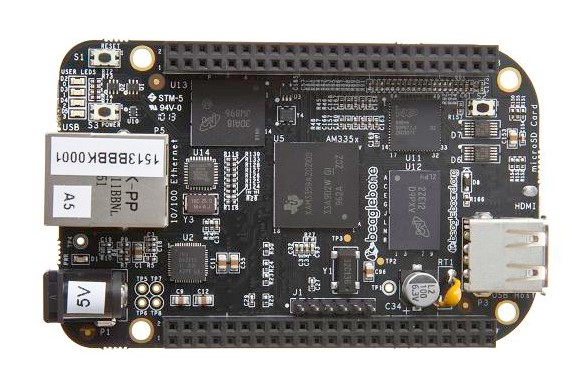
\includegraphics[angle=0,height=5cm]{images/BeagleBoneBlack.jpg}
\caption{Originaler BeagleBone Black}
\label{fig:BeagleBoneBlack}
\end{figure}


\section{Aufgabenstellung}
%Auftrag generell
Im Auftrag des Industriepartners Variosystems soll ein eigener, kostengünstiger und auf dem BeagleBone Black basierter Platinencomputer entwickelt werden. Dafür gilt es, ergänzend zu den eigentlichen Funktionen des BeagleBone Black, weitere Funktionen wie WLAN, Bluetooth Low-Energy, und GSM/GPRS zu integrieren. Zusätzlich soll ein TFT-Display mit einem kapazitivem Multi-Touch-Screen angeschlossen werden, welches von Variosystems zur Verfügung gestellt wird. Das Ganze soll dann als Einheit aufgebaut werden.

%Herstellbarkeit praktisch
Ziel der Arbeit ist es, dass Variosystems diesen Computer selber herstellen und nach Wunsch modifizieren kann. Die Produktionspläne sollen so aufbereitet werden, dass die benötigten PCBs bei einem PCB-Hersteller bestellt werden können. Die Bestückung der PCBs erfolgt dann bei Variosystems. Bei den Bauteilen ist ein besonderes Augenmerk auf die Lieferbarkeit zu werfen. Damit die Bauteile bestellt werden können, muss eine Bauteilliste, auch 'Bill of material' oder kurz BOM, erstellt werden. Diese Liste ist mit der Bestellnummer von üblichen Distributoren wie zum Beispiel Digi-Key oder Mouser zu ergänzen. Standartbauteile, wie etwa Widerstände, hat Variosystems auf Lager. Bei solchen Bauteilen muss auch die Artikelnummer von Variosystems für das entsprechende Bauteil in der BOM aufgeführt werden.

%Modularität, kritischer bereich, 
Die Hardware wie auch die Software sollen möglichst modular aufgebaut sein. Dies bedeutet für die Entwicklung der Hardware, dass alle Bauteile für eine bestimmte Funktion gruppiert und eindeutig erkennbar sein müssen. Ebenso sollen die Bauteile identifiziert werden, welche für die Lauffähigkeit des Computers unbedingt benötigt werden. Ein besonderes Augenmerk ist auf die Stellen zu werfen, bei denen die Leiterbahngeometrie relevant ist. Wie etwa bei der Hochgeschwindigkeitsschnittstelle zwischen Prozessor und RAM. Die Softwaretreiber sollen so geschrieben sein, dass die einzelnen Treiber ohne die anderen lauffähig sind. 

%Software
Zusätzlich zu den Treibern sollten auch Applikationen für die einzelnen Module entwickelt werden. Diese Applikationen sollen als Demonstration der Funktionen und als Vorlage für mögliche Anwendungen verwendet werden können.
